\documentclass[conference]{IEEEtran}
\IEEEoverridecommandlockouts
% The preceding line is only needed to identify funding in the first footnote. If that is unneeded, please comment it out.
\usepackage{cite}
\usepackage[brazil]{babel} % pacote portugues 
\usepackage[utf8]{inputenc} % pacote para acentuacao direta
\usepackage{amsmath,amssymb,amsfonts}
\usepackage{algorithmic}
\usepackage{graphicx}
\usepackage{textcomp}
\usepackage{xcolor}
\usepackage{subcaption}
\def\BibTeX{{\rm B\kern-.05em{\sc i\kern-.025em b}\kern-.08em
    T\kern-.1667em\lower.7ex\hbox{E}\kern-.125emX}}
\begin{document}

\title{BSN - Computação evolucional em \emph{Smart Grid}
%*\\{\footnotesize \textsuperscript{*}Note: Sub-titles are not captured in Xplore and should not be used}
}

\author{\IEEEauthorblockN{1º Daniel Alexandre Oleinik}
\IEEEauthorblockA{\textit{CPGEI - COORD.PROG.POS-GRAD.INFOR.IND.ENG.ELET} \\
\textit{UTFPR - Universidade Tecnológica Federal do Paraná}\\
Curitiba, Brasil}
\and
\IEEEauthorblockN{2º Mauro Sergio Pereira Fonseca}
\IEEEauthorblockA{\textit{CPGEI - COORD.PROG.POS-GRAD.INFOR.IND.ENG.ELET} \\
\textit{UTFPR - Universidade Tecnológica Federal do Paraná}\\
Curitiba, Brasil}
\and
\IEEEauthorblockN{3º Anelise Munaretto}
\IEEEauthorblockA{\textit{CPGEI - COORD.PROG.POS-GRAD.INFOR.IND.ENG.ELET} \\
\textit{UTFPR - Universidade Tecnológica Federal do Paraná}\\
Curitiba, Brasil}
}

\maketitle

\begin{abstract}
O crescente consumo de energia proveniente de fontes não renováveis e finitas tem incentivado o avanço no desenvolvimento e utilização de novas opções de geração de energia. Estas opções, quando incorporadas ao sistema atual de geração e distribuição de energia elétrica, devem demandar novas exigências do sistema de comunicação utilizado entre os equipamentos da rede, motivando o desenvolvimento do \emph{Smart Grid} (SG). O presente documento propõe um método para melhoria e otimização de uma rede, ou grid, de acesso construída em fibra óptica com topologia \emph{mesh}, através de alterações das conexões físicas da rede em conjunto com uma gerência reativa inteligente.
\end{abstract}

\begin{IEEEkeywords}
\emph{Smart Grid}, Chaveador óptico, Redes IP, Redes \emph{Mesh}, Otimização, Latência, Algoritmos Genéticos, Computação Evolucional
\end{IEEEkeywords}

\section{Introdução}
A utilização de combustíveis fósseis, o aquecimento global e o aumento da população mundial têm se tornado tópicos cada vez mais importantes. Estes fatos têm acelerado o desenvolvimento de fontes renováveis de energia, como a eólica e solar, que prometem causar menos impactos ambientais. A integração dessas fontes de energia aos sistemas existentes de distribuição e transmissão, demanda a existência de um novo \emph{grid} de comunicação que ofereça uma infra-estrutura mais rápida, eficiente e confiável \cite{Art-Gungor2013}.

Ainda segundo \cite{Art-Gungor2013}, as tecnologias de energia renovável possuem tendência natural de instalação não centralizada, como os geradores fotovoltaicos ou eólicos, já que ambos aproveitam-se de características geográficas e/ou climáticas. Logo, a utilização destas tecnologias deve transformar o sistema de distribuição de energia atual em um grande sistema de geração distribuída de energia, tornando-se imperativo a utilização de uma infraestrutura capaz de suprir as necessidades de comunicação demandadas pela variedade de sensores, atuadores e elementos utilizados no controle desta nova rede de geração e distribuição de energia. O que, em resumo, representa o próprio conceito de \emph{Smart Grid} (\emph{Smart Grid}).

Este trabalho apresenta resultados de simulações quanto a utilização de chaveadores ópticos em pontos estratégicos da rede (considerando uma infraestrutura de rede construída com fibras ópticas) buscando \emph{by-passar} equipamentos sem prejudicar nenhuma comunicação, resultando em uma otimização em camada 1 da rede considerada com viés em valores de latência.

\section{Proposta}

\subsection{Conceitos Básicos}

\subsubsection{Topologia de Rede \emph{mesh}}
Existem diversas formas de realizar a interconexão entre \emph{hosts}. Segundo \cite{Book-Kurose2013} uma rede de computadores nada mais é do que uma infraestrutura de comunicação que fornece serviços à aplicações distribuídas através de \emph{links} de ``chaveadores de pacotes''. A topologia da rede depende de como esta interconexão é realizada, de maneira geral, podem-se destacar como mais comuns as topologias em barramento, anel, estrela, árvore e malha ou \emph{mesh}.

A topologia \emph{mesh} é caracterizada pela criação de uma rede grandemente (podendo chegar a ser plenamente) interconectada, formando diversos caminhos redundantes para a interligação entre a origem e o destino das mensagens. Fato que confere a este tipo de rede um elevado grau de disponibilidade, visto que mesmo em caso de falha de equipamentos ou da infraestrutura a comunicação não é necessariamente comprometida. A Figura \ref{fig_topologia_multiplo_mesh} ilustra uma rede \emph{mesh}. É possível notar que neste tipo de topologia de rede existem custos atrelados ao roteamento, encaminhamento e processamento de pacotes já que, excluindo-se a situação em que o ponto origem e o destino da comunicação seja vizinhos (diretamente ligados), será invariavelmente necessária a repetição de pacotes por parte de nós intermediários para o estabelecimento da comunicação.

\begin{figure}[htbp]
	\centering
	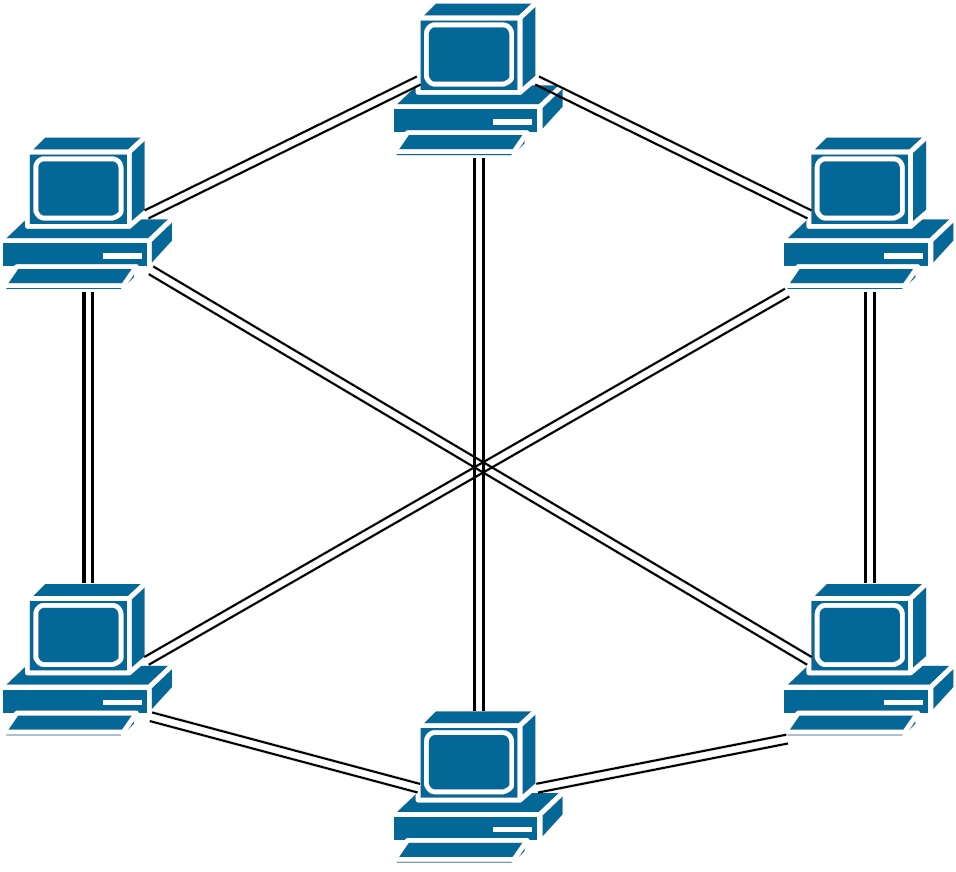
\includegraphics[width=0.15\textwidth]{./figuras/Topologia-Mesh.jpg} % <- formatos PNG, JPG e PDF
	\caption{Topologia em \emph{mesh}.}
	\label{fig_topologia_multiplo_mesh}
\end{figure}

\subsubsection{Chaveador óptico}
A comunicação em redes ópticas é feita através da modulação de sinais luminosos, cada um desses sinais possui uma frequência diferente (usualmente também chamada de cor do sinal) o que implica em diferentes comprimentos de onda. Redes complexas e com grande número de $\lambda$s  como as redes ópticas atuais, possuem em seus nós centrais equipamentos conhecidos como comutadores ópticos, também chamados de \emph{Optical Cross Connect} ou OXC.

Os OXCs podem realizar roteamento interno de sinais de maneira puramente óptica, puramente elétrica ou híbrida \cite{Book-Ramaswami2010}, sendo neste caso chamados de OXC's translúcidos, este tipo de equipamento é amplamente empregado nas redes ópticas atuais e são muitas vezes conhecidos como \emph{Optical-Electrical-Optical} ou Óptico-Elétrico-Óptico em tradução livre. 

Chaveadores ópticos por sua vez são componentes capazes de desviar um feixe luminoso através da utilização de um prisma refletor. A Figura \ref{fig_chaveador_optico} mostra o diagrama interno simplificado de um chaveador óptico, percebe-se que seu funcionamento é análogo ao de um relé elétrico.

\begin{figure}[htbp]
	\centering
	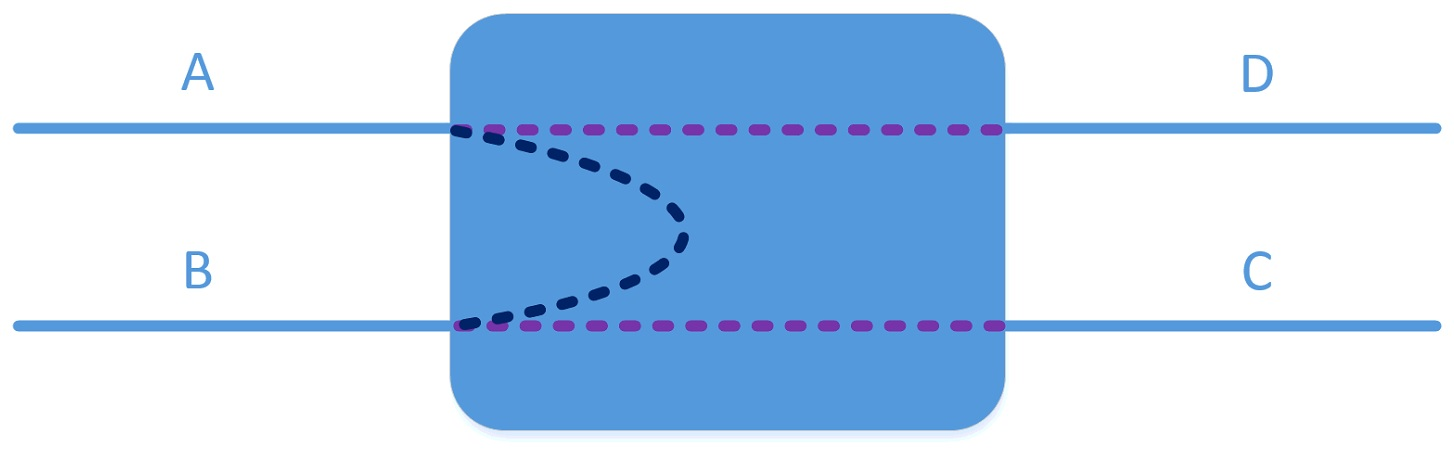
\includegraphics[width=0.3\textwidth]{./figuras/Switch_optico.jpg} % <- formatos PNG, JPG e PDF
	\caption[Exemplo básico chaveador óptico]{Diagrama interno simplificado de um chaveador óptico. Em um estado este componente transmite bidirecionalmente a luz da interface A para D e B para C, quando acionado ele transmite bidirecionalmente a luz da interface A para B. Adaptado de \cite{Accelink2014}}
	\label{fig_chaveador_optico}
\end{figure}

É importante ressaltar que um chaveador óptico é um componente essencialmente passivo. Quando o prisma refletor interno é acionado a luz passa a ser refletida para a saída sem sofrer outro tipo de influência, ou seja, ela é apenas desviada. Entretanto a utilização de um chaveador óptico em um equipamento OEO pode conferir-lhe a capacidade de desviar sinais ópticos caso necessário, surgindo assim um equipamento de roteamento que pode ser classificado como sendo um OXC translúcido. 

\subsubsection{Atrasos em redes ópticas}
Os atrasos existentes em equipamentos elétricos utilizados em redes ópticas têm diversas origens, como o processamento dos dados (intrinsecamente relacionado ao poder de processamento do equipamento) e as conversões de meio necessárias, sendo que para cada equipamento podem-se considerar pelo menos duas dessas conversões (óptica-elétrica-óptica). 

Logo, todas as vezes que um pacote trafega em uma rede óptica acaba sofrendo atrasos, que são traduzidos em forma de latência, em cada um dos nós participantes do circuito. Estes atrasos devem ser somados a fim de determinar a latência total de um enlace. A Figura \ref{fig_latency_link} mostra a acúmulo da latência através de um enlace óptico entre dois pontos. 

\begin{figure} [htbp]% normalmente utilizar [!t]
	\centering
	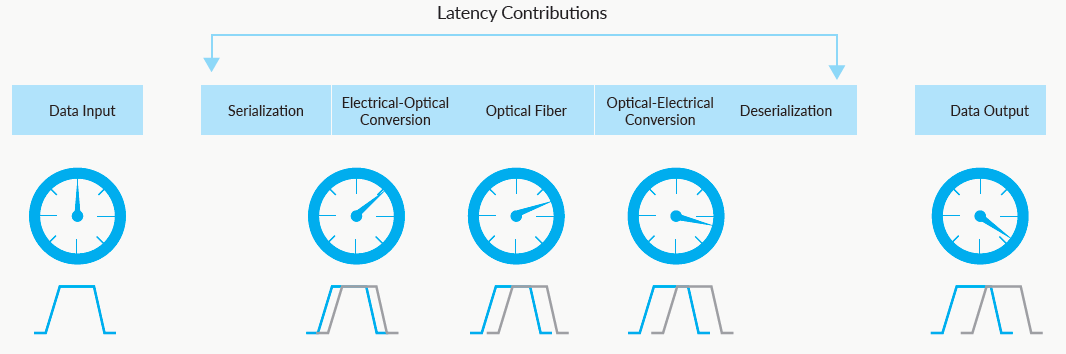
\includegraphics[width=0.4\textwidth]{./figuras/latency-link.png}
	\caption[Latência de Link]{Latência em comunicação entre dois pontos utilizando link óptico. Os principais pontos de inserção de latência na comunicação são resultantes dos processos de conversão elétrica-óptica, transmissão de dados, conversão óptica-elétrica e disponibilização dos dados no destino (desserialização e processamento). Fonte \cite{Art-Coffe2017}}
	\label{fig_latency_link}
\end{figure}

\subsubsection{\emph{Smart Grids} de Distribuição de Energia}
As \emph{Smart Grids} oferecem uma ampla variedade de serviços até então minoritários ou inexistentes nas redes de distribuição de energia convencionais. Em \cite{Art-Ma2013} pode-se encontrar um breve relato de alguns dos benefícios oferecidos pelas redes inteligentes como o melhor gerenciamento de energia, monitoramento remoto da operação e assertividade na recuperação diante de falhas, diminuição de desperdício através do maior controle entre ajuste de produção e demanda, menor necessidade de equipes de campo, entre outros. A Tabela \ref{tab_comparacao_grids} compara os principais pontos de diferença entre as redes de distribuição de energia atuais e as \emph{Smart Grids}.

\begin{table}[tbp]
\begin{tabular}{l|l|l|}
\cline{2-3}
 & \multicolumn{1}{c|}{\textbf{Grid Atual}} & \multicolumn{1}{c|}{\textbf{Smart Grid}} \\ \hline
\multicolumn{1}{|l|}{\textbf{Fluxo de informação}} & Unidirecional & Bidirecional \\ \hline
\multicolumn{1}{|l|}{\textbf{Geração de eletricidade}} & Geração centralizada & Geração Distribuída \\ \hline
\multicolumn{1}{|l|}{\textbf{Topologia do GRID}} & Radial & \emph{Mesh} \\ \hline
\multicolumn{1}{|l|}{\textbf{Sensores}} & Poucos sensores & Muitos sensores \\ \hline
\multicolumn{1}{|l|}{\textbf{Monitoramento}} & Usualmente inexistente & Auto monitorada \\ \hline
\multicolumn{1}{|l|}{\textbf{Recuperação de falha}} & Restauração manual & Auto reconfiguração \\ \hline
\multicolumn{1}{|l|}{\textbf{Teste}} & Manual & Remota \\ \hline
\multicolumn{1}{|l|}{\textbf{Capacidade de controle}} & Limitado & Penetrante \\ \hline
\multicolumn{1}{|l|}{\textbf{Tipo de controle}} & Passivo & Ativo \\ \hline
\multicolumn{1}{|l|}{\textbf{Eficiência}} & Baixa & Alta \\ \hline
\multicolumn{1}{|l|}{\textbf{Geração de poluição}} & Alta & Baixa \\ \hline
\end{tabular}
\caption[Comparação entre GRIDS normal e \emph{Smart}]{Comparação elencando os parâmetros básicos de rede entre uma rede de distribuição normal e uma rede \emph{Smart Grid}. Fonte: adaptado de \cite{Art-Ma2013}}
\label{tab_comparacao_grids}
\end{table}
	
\subsection{BSN - \emph{Bypass} Seletivo de Nós}
O BSN foi especificamente desenvolvido para otimização de latência em redes ópticas através da utilização de chaveadores ópticos em pontos estratégicos da rede, ou seja, através da manipulação do \emph{layer} físico da rede e consequentemente da topologia da mesma. Dessa forma equipamentos em posições específicas da rede podem ser desviados sem a necessidade de nenhuma conversão de meio ou mesmo de processamento, resultando na mínima inserção de latência possível. 

O BSN opera de maneira completamente independente do protocolo de roteamento utilizado na rede em questão visto que altera somente a topologia da mesma, podendo ser usado inclusive em conjunto com protocolos de camada 2. Os pontos da rede de acionamento do chaveador óptico podem ser escolhidos em ramos de um grafo com muitos vértices (\emph{hops}) ou podem ser planejados para o estabelecimento de rotas específicas para comunicação com pontos críticos do sistema, estabelecendo um \emph{Service Level Agreement} em \emph{layer} físico. Através da sua utilização é possível reduzir o grafo da rede possibilitando uma nova configuração de conexões inexistente na rede original e consequentemente uma nova variedade de rotas possíveis.

Cada vez que o BSN ativa um \emph{bypass}, as duas arestas envolvidas são unificadas evitando o vértice das mesmas, criando assim um novo grafo com uma distância entre os dois vértices finais de um vértice a menos, como representado na Figura \ref{fig-bypass-exemplo}.

\begin{figure}[htbp]
	\centering
	\begin{subfigure}[t]{0.2\textwidth}
		\centering
		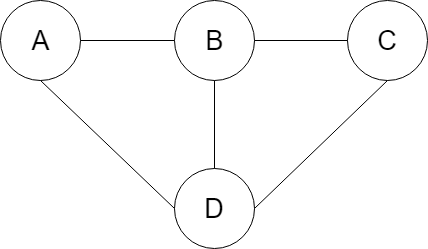
\includegraphics[width=0.9\textwidth]{./figuras/Bypass-exemplo-A.png} % <- formatos PNG, JPG e PDF
		\caption{Chaveador óptico desativado}
		\label{fig_bypass_exemplo_A}
	\end{subfigure}%
	~
	\begin{subfigure}[t]{0.2\textwidth}
		\centering
		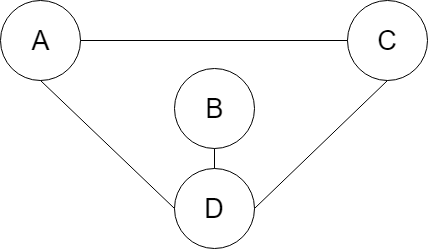
\includegraphics[width=0.9\textwidth]{./figuras/Bypass-exemplo-B.png} % <- formatos PNG, JPG e PDF
	\caption{Chaveador óptico ativado}
	\label{fig_bypass_exemplo_B}
	\end{subfigure}
	\caption[Exemplo de atuação de \emph{by-pass} óptico]{Efeito da utilização do chaveador ótico em uma rede de comunicação. Em \ref{fig_bypass_exemplo_A} pode-se ver a rede original contendo dois saltos entre os vértices A e C. Em \ref{fig_bypass_exemplo_B} após o acionamento do dispositivo no vértice B pode-se ver e existência de apenas um salto entre os vértices A e C}
	\label{fig-bypass-exemplo}
\end{figure}

\subsubsection{Funcionamento}
Para avaliar o funcionamento do BSN foi gerada a rede da Figura \ref{BSN-example-network}, representada por um grafo simples com valência igual a 3 e topologia \emph{mesh}. Este grafo foi submetido ao protocolo STP para cálculo dos caminhos ótimos para todos os vértices à partir do vértice origem (arbitrariamente escolhido como sendo o 1). O resultado, apresentado na Figura \ref{BSN-example-network-tree}, é na verdade o \emph{minimal spanning tree} para o grafo da Figura \ref{BSN-example-network}.

O mesmo grafo da Figura \ref{BSN-example-network}, foi submetido à execução do BSN. Como resultado decidiu-se pelo acionamento do chaveador óptico no vértice 7, interligando o vértice 1 diretamente ao 4 gerando um novo grafo representado na Figura \ref{BSN-example-opt-switch}. Este grafo, quando submetido ao cálculo dos caminhos ótimos também utilizando o protocolo STP, resulta na Figura \ref{BSN-example-rede-otimizada}, onde pode-se notar a diminuição da profundidade em comparação com aquele mostrado na Figura \ref{BSN-example-network-tree}.

\begin{figure}[t!]
	\centering
	\begin{subfigure}[t]{0.2\textwidth}
		\centering
		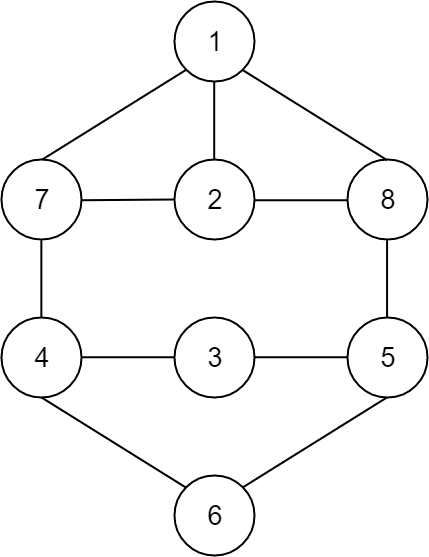
\includegraphics[width=0.7\textwidth]{./figuras/BSN-ex-network-generation.png} % <- formatos PNG, JPG e PDF
		\caption{Rede gerada}
		\label{BSN-example-network}
	\end{subfigure}%
	~
	\begin{subfigure}[t]{0.2\textwidth}
		\centering
		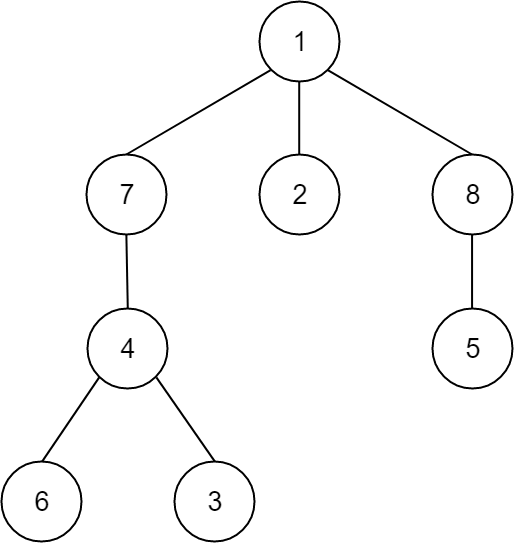
\includegraphics[width=0.7\textwidth]{./figuras/BSN-ex-network-generation-tree.png} % <- formatos PNG, JPG e PDF
	\caption{Árvore da Rede}
	\label{BSN-example-network-tree}
	\end{subfigure}
	~
	\begin{subfigure}[t]{0.2\textwidth}
		\centering
		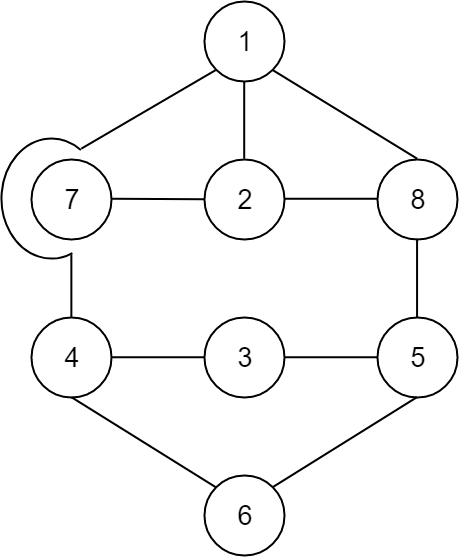
\includegraphics[width=0.7\textwidth]{./figuras/BSN-ex-bypass.png} % <- formatos PNG, JPG e PDF
	\caption{Chaveador óptico ativado}
	\label{BSN-example-opt-switch}
	\end{subfigure}
	~
	\begin{subfigure}[t]{0.2\textwidth}
		\centering
		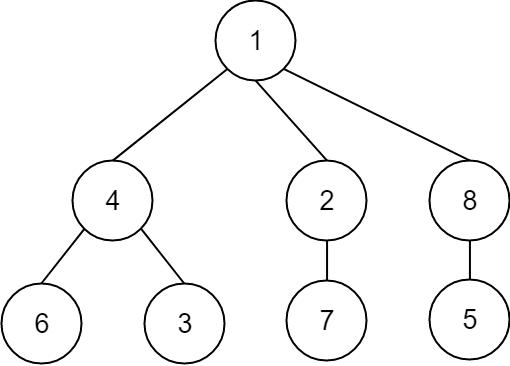
\includegraphics[width=0.7\textwidth]{./figuras/BSN-ex-network-final.png} % <- formatos PNG, JPG e PDF
	\caption{Rede resultante}
	\label{BSN-example-rede-otimizada}
	\end{subfigure}
	\caption[Exemplo de funcionamento do BSN]{Exemplo de funcionamento do BSN. Percebe-se que o BSN consegue reduzir a profundidade de uma rede gerando uma nova possibilidade de conexões através da manipulação da camada física da mesma.}
	\label{fig-bsn-exemplo}
\end{figure}

É possível notar que a profundidade da rede, ligada diretamente à latência da comunicação, é reduzida impactando na redução de latência para a comunicação entre os nós envolvidos. Para o exemplo em questão pode-se reduzir a profundidade máxima da rede de 3 saltos para 2 (33,33\%), consequentemente impactando diretamente na latência devido a ausência de conversão de meio assim como processamento no vértice desviado, conforme descrito na Figura \ref{fig_latency_link}. 

\subsubsection{Custos de rede total e individual}
O custo de rede total é definido como a soma de todos os custos individuais (número de saltos) para comunicação em cada um dos \emph{links} da rede. Logo, utilizando a rede de exemplo representada na Figura \ref{BSN-example-network-tree} tem-se o mostrado na Tabela \ref{tab-custo-rede-BSN-example-network-tree} como sendo os custos individuais para comunicação entre o nó origem e os demais assim como o custo total da rede. Em contrapartida, ao utilizar a rede representada na Figura \ref{BSN-example-rede-otimizada}, que foi otimizada através da utilização do BSN, tem-se como resultado para os custos individuais e custo total o representado na Tabela \ref{tab-custo-rede-bsn-otimizada}.

\begin{table}[t!]
	\centering
		%\begin{table}[]
			\begin{tabular}{llllll}
			\hline
			\multicolumn{1}{|l|}{\textbf{Nó destino}} & \multicolumn{4}{c}{\textbf{Caminho}} & \multicolumn{1}{c|}{\textbf{Custo}} \\ \hline
			\multicolumn{1}{|l|}{\textbf{2:}} & 1 & 2 &  & \multicolumn{1}{l|}{} & \multicolumn{1}{l|}{1} \\ \hline
			\multicolumn{1}{|l|}{\textbf{3:}} & 1 & 7 & 4 & \multicolumn{1}{l|}{3} & \multicolumn{1}{l|}{3} \\ \hline
			\multicolumn{1}{|l|}{\textbf{4:}} & 1 & 7 & 4 & \multicolumn{1}{l|}{} & \multicolumn{1}{l|}{2} \\ \hline
			\multicolumn{1}{|l|}{\textbf{5:}} & 1 & 8 & 5 & \multicolumn{1}{l|}{} & \multicolumn{1}{l|}{2} \\ \hline
			\multicolumn{1}{|l|}{\textbf{6:}} & 1 & 7 & 4 & \multicolumn{1}{l|}{6} & \multicolumn{1}{l|}{3} \\ \hline
			\multicolumn{1}{|l|}{\textbf{7:}} & 1 & 7 &  & \multicolumn{1}{l|}{} & \multicolumn{1}{l|}{1} \\ \hline
			\multicolumn{1}{|l|}{\textbf{8:}} & 1 & 8 &  & \multicolumn{1}{l|}{} & \multicolumn{1}{l|}{1} \\ \hline
			 & \multicolumn{4}{l}{\textbf{Custo Total}} & \textbf{13}
			\end{tabular}
		\caption{Calculo de custo - Rede Figura \ref{BSN-example-network-tree}}
		\label{tab-custo-rede-BSN-example-network-tree}
		%\end{table}
\end{table}
		
\begin{table}[t!]
	\centering
			%\begin{table}[]
			\begin{tabular}{lllll}
			\hline
			\multicolumn{1}{|l|}{\textbf{Nó destino}} & \multicolumn{3}{c}{\textbf{Caminho}} & \multicolumn{1}{c|}{\textbf{Custo}} \\ \hline
			\multicolumn{1}{|l|}{\textbf{2:}} & 1 & 2 & \multicolumn{1}{l|}{} & \multicolumn{1}{l|}{1} \\ \hline
			\multicolumn{1}{|l|}{\textbf{3:}} & 1 & 4 & \multicolumn{1}{l|}{3} & \multicolumn{1}{l|}{2} \\ \hline
			\multicolumn{1}{|l|}{\textbf{4:}} & 1 & 4 & \multicolumn{1}{l|}{} & \multicolumn{1}{l|}{1} \\ \hline
			\multicolumn{1}{|l|}{\textbf{5:}} & 1 & 8 & \multicolumn{1}{l|}{5} & \multicolumn{1}{l|}{2} \\ \hline
			\multicolumn{1}{|l|}{\textbf{6:}} & 1 & 4 & \multicolumn{1}{l|}{6} & \multicolumn{1}{l|}{2} \\ \hline
			\multicolumn{1}{|l|}{\textbf{7:}} & 1 & 2 & \multicolumn{1}{l|}{7} & \multicolumn{1}{l|}{2} \\ \hline
			\multicolumn{1}{|l|}{\textbf{8:}} & 1 & 8 & \multicolumn{1}{l|}{} & \multicolumn{1}{l|}{1} \\ \hline
			 & \multicolumn{3}{l}{\textbf{Custo Total}} & \textbf{11}
			\end{tabular}
	\caption{Calculo de custo - Rede Figura \ref{BSN-example-rede-otimizada}}
	\label{tab-custo-rede-bsn-otimizada}
	%\end{table}
	\label{tab_calc_custo}
\end{table}

À partir da comparação dos dados apresentados nas Tabelas \ref{tab-custo-rede-BSN-example-network-tree} e \ref{tab_calc_custo} nota-se que o custo total da rede foi otimizado em aproximadamente 15,4\% sendo que para os destinos 3 e 6 foi alcançado 33,33\% e para os destinos 4 e 7 50\% de melhoria.

\subsubsection{Implementação}
O algoritmo do BSN é baseado em computação evolucional. A estratégia de otimização utilizada envolve a representação da rede através de um vetor onde cada posição representa um dos nós e seu valor representa a ativação do respectivo chaveador óptico. Este vetor é então considerado como um cromossomo e utilizado em um algoritmo genético que busca minimizar a função de \emph{fitness} do problema, que pode ser traduzida como o custo total da rede. 

Consequentemente, para que o custo total seja reduzido, é necessário que os custos individuais sejam reduzidos, sendo natural que os ramos mais compridos (com maior custo) do grafo sejam os mais impactados. Dessa forma, apesar de o objetivo final ser a otimização de latência para a rede como um todo, é possível adequar a função de \emph{fitness} do algoritmo para refletir a otimização preferencialmente para destinos com alta latência ou maior prioridade.

\subsection{Resultados}

\subsubsection{Melhoria de Custo total}
Para avaliação da performance do BSN foram utilizadas redes criadas aleatoriamente de 5 a 100 nós com passo incremental de 5 unidades, ou seja, foram geradas redes de 5, 10, 15 e assim sucessivamente até 100 nós. A partir dos resultados conseguidos utilizando 300 redes diferentes, foi gerado um gráfico do percentual de melhoria de custo total representado na Figura \ref{fig_graph_bsn_medio_all}, cujo intervalo de confiança utilizado é de 98\%.

\begin{figure} [ht]% normalmente utilizar [!t]
	\centering
	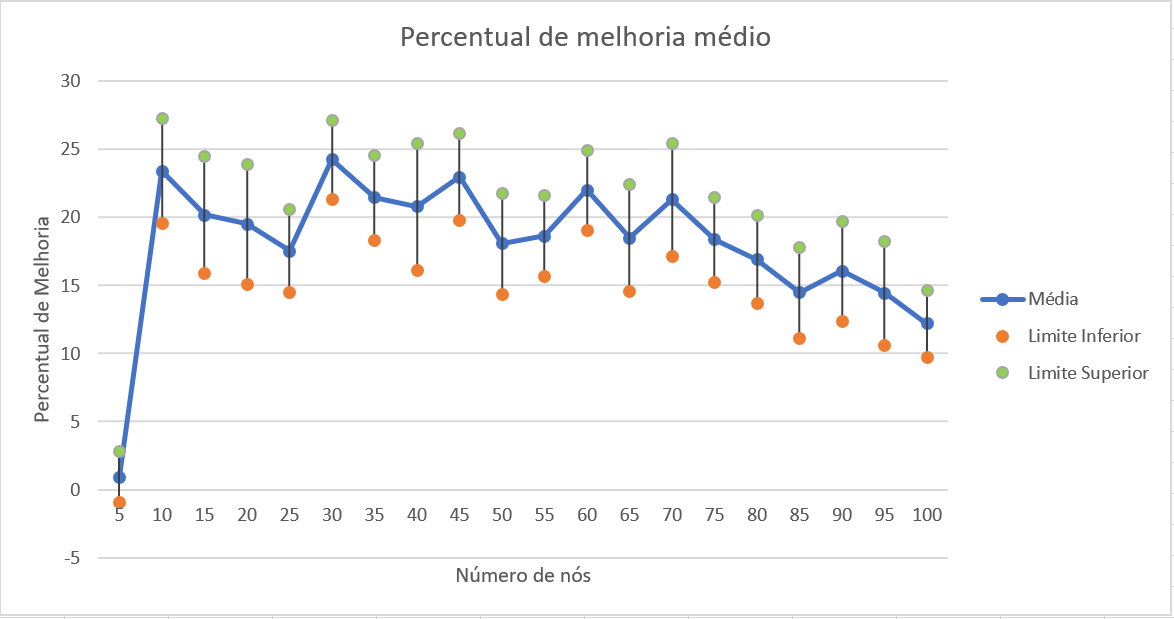
\includegraphics[width=0.49\textwidth]{./figuras/BSN-resultados-medios-all2.png} % <- formatos PNG, JPG e PDF
	\caption[Melhoria de custo x tamanho de rede]{Gráfico percentual comparativo de resultados médios de melhoria de custo total entre redes de diferentes tamanhos considerando um intervalo de confiança de 98\%.}
	\label{fig_graph_bsn_medio_all}
\end{figure}

\subsubsection{Melhoria de Custo individual}
Ao analisar os custos individuais das redes utilizadas na geração do gráfico mostrado na Figura \ref{fig_graph_bsn_medio_all} chega-se no gráfico apresentado na Figura \ref{fig_graph_melhoria_por_custo}. Aqui pode-se notar claramente uma significativa e crescente melhora no custo das rotas atrelado ao aumento das mesmas. Ou seja, quanto maior a rota, maior a otimização resultante.

Considerando um ramo de rede hipotético com 100 saltos na topologia original, pode-se prever que após a utilização do BSN este mesmo ramo resulte em um novo caminho com aproximadamente 73 saltos, representando uma redução de 27\% em relação à topologia original. Em outras palavras, pontos da cidade que não poderiam originalmente ser atendidos pelo SG devido à distância com relação ao centro de controle, podem passar a ser considerados como alcançáveis já que a latência deve ser significativamente reduzida, representando grande economia para a distribuidora de energia em questão.

\begin{figure} [ht]% normalmente utilizar [!t]
	\centering
	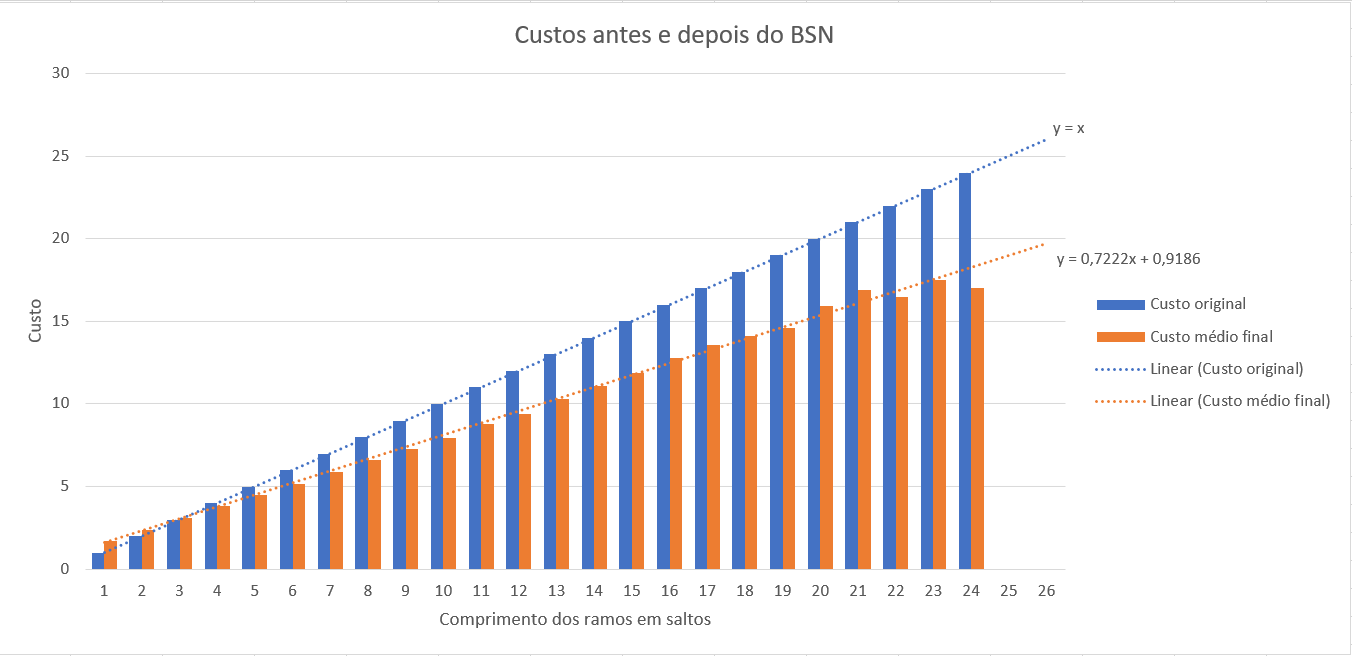
\includegraphics[width=0.49\textwidth]{./figuras/Melhoria-por-custo.png} % <- formatos PNG, JPG e PDF
	\caption[Custo antes e depois do BSN]{Gráfico comparativo de resultados médios de melhoria de custo individual para cada rota.}
	\label{fig_graph_melhoria_por_custo}
\end{figure}


\section{Conclusão}
Através da utilização do BSN pode-se notar uma sensível melhora nos parâmetros de custo/profundidade da rede resultante em detrimento de sua largura quando comparada ao grafo da rede original. Em outras palavras, o BSN tem a capacidade de converter uma rede profunda em uma rede larga, obviamente sujeito às limitações de conexão já existentes na rede original.

Através da análise da Figura \ref{fig_graph_bsn_medio_all} fica claro uma diminuição de efetividade da metodologia na melhoria do custo total da rede quando usado em redes com muitos nós. Considerando que o custo total é dado pela soma de todos os custos entre o nó central e todos os destinos da rede, espera-se apenas algumas conexões com grandes valores de custo, ou seja, a rede deve possuir muito mais conexões com baixo custo do que com alto custo. Desta forma a contribuição da otimização destes ramos para o custo total acaba sendo pequena. Além disso, quanto mais nós existirem em uma rede \emph{mesh}, maior será a possibilidade de combinações/rotas disponíveis. Desta forma, em uma rede com alto nível de multipercursos espera-se que as rotas ótimas já possuam baixo custo mesmo sem alteração de topologia.

Em contrapartida o mesmo não se aplica ao considerar-se o custo individual de cada um dos ramos, o que em geral representa a maior preocupação deste tipo de aplicação. Conforme o apresentado em \ref{fig_graph_melhoria_por_custo}, quando maior o número de saltos de um ramo , o que representa o real gargalo da rede SG, maior será o percentual de melhoria após a utilização do BSN.

Como consequência secundária, mas não menos importante, a utilização da proposta pode permitir que pontos anteriormente fora da SG devido à distância possam ser incluídos sem a necessidade de construção de um centro de controle de rede secundário. Acarretando em maior abrangência e grande economia para a distribuidora de energia elétrica.



\bibliographystyle{IEEEtran}
\bibliography{IEEEabrv,SMMC2018}


\end{document}
